\section{Presentazione}
    Per la presentazione del sito abbiamo utilizzato il linguaggio CSS usufruendo quasi esclusivamente di misure relative come em e percentuali e cercando di ridurre al minimo l'utilizzo di misure statiche come i px per creare un design fluido e che sia facilmente usufruibile da mobile.
    Così facendo siamo riusciti ad ottenere un sito accessibile su ogni dispositivo, grazie anche all'utilizzo di media query che vanno a rendere il design del sito scalabile e accessibile.
    
    \subsection{Presentazione Generale}
    Questa breve sezione descriverà quello che è lo scheletro comune a tutte le pagine del sito.
    Tutte le pagine presentano, uno sfondo giallastro nella parte esterna al body, il logo della concessionaria in cima alla pagina con la possibilità di cliccarlo per venire reindirizzati alla home, appeno sotto di esso si potrà trovare il menu. Il menù è strutturato nella forma classica con una visualizzazione orizzontale di tutte le voci principali, la presentazione del menu cambierà quando utilizzato da mobile(vedere sezione "Differenze mobile vs desktop"). In fondo alla pagina si potrà infine trovare il footer che ha il principale compito di contenere la dicitura per il copyright.

    \subsection{Principali differenze mobile vs desktop}
    Le seguenti sezioni delineeranno le differenze più importanti che si possono osservare nella struttura delle pagine mobile rispetto alla loro controparte desktop, queste modifiche sono state implementate con l'intento di garantire una visualizzazione facile e pulita del sito da mobile.

        \subsubsection{Menu mobile}
        Le voci del menu saranno nascoste, per visualizzarle basterà cliccare sul burger menu in alto a destra ed esse compariranno in un menu a tendina.

        \subsubsection{Home mobile}
        Nella Home l'immagine della concessionaria non viene più visualizzata affianco al testo ma sopra di esso.

        \subsubsection{Veicoli a noleggio e Veicoli in vendita mobile}
        I vari filtri di ricerca per le auto verranno visualizzati in blocchi quindi ognuno occuperà un intera riga inclusi il bottone per il submit è quello per ricaricare la pagina.

        \subsubsection{Area personale ed Area amministratore}
        Il menu utente ed il menu amministratore non saranno più alla sinistra del contenuto ma sopra di esso.
    
    \subsection{CSS Print}
        Il compito di gestire la presentazione della maggior parte delle pagine durante la stampa è stato affidato al file cssPrint.css, esso elimina tutti gli elementi visivi non necessari durante una stampa come il logo, il footer, i menu, i colori di background e le immagini che non hanno valore informativo in modo da ottenere un stampa il più efficiente possibile.
        Vi sono inoltre alcune pagine a cui sono stati dedicati dei fogli di stile aggiuntivi per gestire situazioni di stampa a loro specifiche.

    \begin{center}
        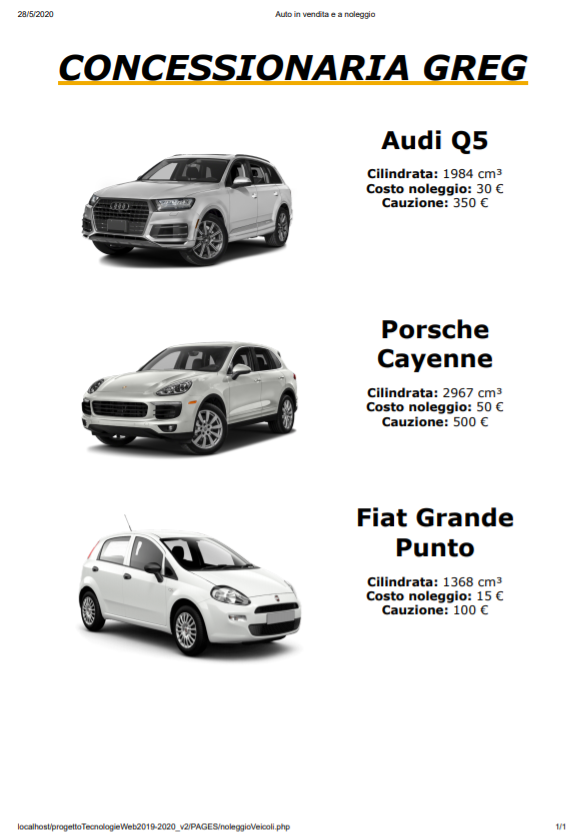
\includegraphics[width=18pc]{./img/StampaVeicoliNoleggio.png}
        \captionof{figure}{Stampa della pagina "Veicoli a noleggio"}
    \end{center}

\pagebreak